\documentclass[a5paper,headsepline,titlepage,11pt,nnormalheadings,DIVcalc]{scrbook}
\usepackage[a5paper,backref]{hyperref}
\usepackage[papersize={165mm,215mm},twoside,bindingoffset=0.5cm,hmargin={2cm,2cm},
				vmargin={2cm,2cm},footskip=1.1cm,driver=dvipdfm]{geometry}
%\usepackage{palatino}
\usepackage{graphicx}
\usepackage{wrapfig}
\usepackage[bahasa]{babel}
\usepackage{fancyhdr}
\usepackage{longtable}
\usepackage{hhline,multirow}
\usepackage{pst-node}

%\setlength{\voffset}{0.5in}
%\setlength{\oddsidemargin}{28pt}
%\setlength{\evensidemargin}{0pt}
\renewcommand{\footrulewidth}{0.5pt}
\lhead[\fancyplain{}{\thepage}]%
      {\fancyplain{}{~}}
\rhead[\fancyplain{}{~}]%
      {\fancyplain{}{\thepage}}
\pagestyle{fancy}
\lfoot[\emph{APP 2010 pertemuan V}]{}
\rfoot[]{\emph{Lingkungan St Petrus Maguwo}}
\cfoot{}

\newcommand{\BU}[1]{\begin{itemize} \item[U:] #1 \end{itemize}}
\newcommand{\BI}[1]{\begin{itemize} \item[I:] #1 \end{itemize}}
\newcommand{\BP}[1]{\begin{itemize} \item[P:] #1 \end{itemize}}
\newcommand{\BPP}[1]{\begin{itemize} \item[Bpk:] #1 \end{itemize}}
\newcommand{\BPW}[1]{\begin{itemize} \item[Ibu:] #1 \end{itemize}}
\title{APP 2010 Pertemuan V\\ Lingkungan St. Petrus}
\author{Wilayah Yohanes De Britto \\Stasi Maguwo \\Paroki Kalasan}
\date{2010}
\hyphenation{a-kan}
\hyphenation{ba-gi-mu}
\hyphenation{ber-a-da}
\hyphenation{ber-du-a}
\hyphenation{be-ri-kan}
\hyphenation{ber-ka-ta}
\hyphenation{ber-nya-nyi}
\hyphenation{ber-sa-ma}

\hyphenation{dah-syat}
\hyphenation{DA-RAH-KU}
\hyphenation{da-tang}
\hyphenation{di-ka-ta-kan}
\hyphenation{di-pim-pin}
\hyphenation{di-se-rah-kan}
\hyphenation{di-tum-pah-kan}

\hyphenation{Eng-kau}
\hyphenation{ha-dap-an}
\hyphenation{han-tar-kan-lah}
\hyphenation{ha-rap-an}

\hyphenation{ja-lan}
\hyphenation{ja-ngan-lah}

\hyphenation{ka-nak}
\hyphenation{ka-re-na}
\hyphenation{kau-lim-pah-kan}
\hyphenation{Kau-cip-ta-kan}
\hyphenation{ke-bang-kit-an-Nya}
\hyphenation{ke-da-tang-an}
\hyphenation{ke-da-tang-an-Nya}
\hyphenation{ke-dua}
\hyphenation{ke-na-ik-kan-nya}
\hyphenation{ke-pa-daMu}
\hyphenation{ke-ra-him-an}
\hyphenation{ke-se-jah-te-ra-an-mu}
\hyphenation{ko-men-tar}

\hyphenation{la-ma-nya}
\hyphenation{lim-pah-kan}

\hyphenation{ma-nu-sia}
\hyphenation{me-nga-da-kan}
\hyphenation{me-ngan-dung-lah}
\hyphenation{me-ngu-kuh-kan}
\hyphenation{me-la-lui}
\hyphenation{me-lim-pah-kan}
\hyphenation{me-lu-hur-kan}
\hyphenation{me-me-cah-me-cah-kan}
\hyphenation{mem-per-sem-bah-kan}
\hyphenation{me-nan-da-ta-ngan-i}
\hyphenation{men-cin-tai}
\hyphenation{meng-a-lir-kan}
\hyphenation{me-nga-sihi}
\hyphenation{me-nge-lu-ar-kan}
\hyphenation{meng-u-cap-kan}
\hyphenation{meng-ung-kap-kan}
\hyphenation{me-num-buh-kan}
\hyphenation{me-nya-ta-kan}
\hyphenation{me-nye-la-mat-kan}
\hyphenation{me-nye-rah-kan}
\hyphenation{me-nye-rah-kanNya}
\hyphenation{me-ra-ya-kan}

\hyphenation{o-rang}
\hyphenation{o-rang-o-rang}

\hyphenation{pa-sang-kan-lah}
\hyphenation{pa-tut}
\hyphenation{pe-ne-ri-ma-an}
\hyphenation{pe-ngam-pun-an}
\hyphenation{Pe-ngan-ta-ra}
\hyphenation{peng-hi-bur-an}
\hyphenation{per-bu-at-an-nya}
\hyphenation{per-ka-ta-an}
\hyphenation{per-ka-win-an}
\hyphenation{per-ni-kah-an}
\hyphenation{per-se-ku-tu-an}
\hyphenation{per-sem-bah-an}
\hyphenation{rom-bong-an}

\hyphenation{se-la-ma}
\hyphenation{se-ka-li-an}
\hyphenation{se-pan-jang}
\hyphenation{se-ra-ya}
\hyphenation{Su-dar-yan-to}

\hyphenation{te-ta-pi}
\hyphenation{ta-ngan-Mu}
\hyphenation{Tu-han}
\hyphenation{tu-lang}
\hyphenation{tu-lang-tu-lang}

\hyphenation{u-mat-Mu}
\hyphenation{wa-kil}

\hyphenation{ba-gi-mu}
\hyphenation{di-se-rah-kan}
\hyphenation{me-la-lui}
\hyphenation{ka-nak}
\hyphenation{ka-re-na}
\hyphenation{ber-ka-ta}
\hyphenation{te-ta-pi}
\hyphenation{per-ka-win-an}
\hyphenation{pa-tut}
\hyphenation{me-lu-hur-kan}
\hyphenation{ber-nya-nyi}
\hyphenation{di-tum-pah-kan}
\hyphenation{pe-ngam-pun-an}
\hyphenation{ber-a-da}
\hyphenation{kau-lim-pah-kan}
\hyphenation{ke-bang-kit-an-Nya}
\hyphenation{per-ka-ta-an}
\hyphenation{pa-sang-kan-lah}
\hyphenation{DA-RAH-KU}
\hyphenation{ke-na-ik-kan-nya}
\hyphenation{per-sem-bah-an}
\hyphenation{per-se-ku-tu-an}


\renewcommand*\thesection{\arabic{section}.}
\setlength{\parindent}{0mm} 

\begin{document}
\thispagestyle{empty}
%\maketitle
%\newsavebox\IBox
%\sbox\IBox{\includegraphics[scale=0.4]{Saint-Peter-Apostle-e.eps}}

\psset{unit=1in}
\begin{pspicture}(4in,6.0in)
% set up the fonts we use
\DeclareFixedFont{\PT}{T1}{ppl}{b}{it}{0.4in}
\DeclareFixedFont{\PTsmall}{T1}{ppl}{b}{it}{0.3in}
\DeclareFixedFont{\PTsmallest}{T1}{ppl}{b}{it}{0.2in}
\DeclareFixedFont{\PTtext}{T1}{ppl}{b}{it}{11pt}
\DeclareFixedFont{\Logo}{T1}{pbk}{m}{n}{0.2in}
% place the front cover picture
%\rput[cb](2.3,2.5){\usebox\IBox}
% put the text on the front cover
\rput[cb](2.5,5.3){\PTsmall {APP 2010}}
\rput[cb](2.5,4.8){\PTsmall {Pertemuan ke V}}
\rput[cb](2.5,1.1){\PTsmall {Lingkungan St. Petrus}}
\rput[cb](2.5,0.6){\PTsmallest {Wilayah Yohanes de Britto}}
\rput[cb](2.5,0.3){\PTsmallest {Stasi Maguwo}}
\rput[cb](2.5,0.0){\PTsmallest {Paroki Marganingsih Kalasan }}

%\rput[cb](3,-1){\PTsmallest {\namagereja}} 

\end{pspicture}
%\tableofcontents 
\newpage
\thispagestyle{empty}
{~}
\newpage
\setlength{\parskip}{2mm}
\section*{Ibadat Tobat}
\subsection*{Nyanyian Pembuka}
\subsection*{Salam Pembuka dan Pengantar}
\BP{Dalam nama Bapa, Putra, dan Roh Kudus}
\BU{Amin.}
Ibu, Bapak, dan Saudara sekalian pada malam hari ini kita sampai pada
pertemuan kelima dari seri APP 2010 yang bertema ’Bersyukur dengan
bertobat dan berbagi berkat’. Pertemuan kali ini akan terdiri atas 2
bagian yaitu bagian pertama berupa ibadat tobat sedang bagian kedua
adalah rencana aksi untuk satu tahun ini.
Ibadat tobat akan diisi renungan yang diharapkan dapat membantu Bapak,
Ibu, dan Saudara untuk lebih mendalami arti bertobat. Bapak,
Ibu, dan Saudara semua diharapkan dapat menuangkan ide dan rencana
pada bagian kedua nanti.
\subsection*{Doa Pembuka}
Allah Bapa Maharahim dan Penuh Belas Kasih, kami bersujud menghadap
hadiratMu dengan segala kerendahan hati. Kami adalah umatMu
yang berdosa, bagaikan anak yang hilang. Namun kami percaya sebelum
kami bertobat Engkau telah terlebih dahulu mendekati kami dan mencari
kami. Berkat kehadiran Kristus PuteraMu, yang telah mengalirkan
darah dan air, terbukalah samudera kerahiman bagi segenap dunia.
Bukalah hati kami untuk mendengarkan SabdaMu dan tergerak untuk
mengikutiMu, demi Kristus Tuhan dan Pengantara kami. Amin.

\subsection*{Bacaan Sabda Tuhan: Luk 15:1-3,11b-24}
\begin{enumerate}
\item Para pemungut cukai dan orang-orang berdosa biasanya datang
kepada Yesus untuk mendengarkan Dia.
\item Maka bersungut-sungutlah orang-orang Farisi dan ahli-ahli Taurat,
katanya: ”Ia menerima orang-orang berdosa dan makan bersama-sama
dengan mereka.”
\item Lalu Ia mengatakan perumpamaan ini kepada mereka:
%% \item ”Siapakah di antara kamu yang mempunyai seratus ekor domba,
%% dan jikalau ia kehilangan seekor di antaranya, tidak meninggalkan
%% yang sembilan puluh sembilan ekor di padang gurun dan pergi
%% mencari yang sesat itu sampai ia menemukannya?
%% \item Dan kalau ia telah menemukannya, ia meletakkannya di atas bahunya
%% dengan gembira,
%% \item dan setibanya di rumah ia memanggil sahabat-sahabat dan tetangga-tetangganya serta berkata kepada mereka: Bersukacitalah bersama-sama
%% dengan aku, sebab dombaku yang hilang itu telah kutemukan.
%% \item Aku berkata kepadamu: Demikian juga akan ada sukacita di sorga
%% karena satu orang berdosa yang bertobat, lebih dari pada sukacita
%% karena sembilan puluh sembilan orang benar yang tidak memerlukan
%% pertobatan.”
%% \item ”Atau perempuan manakah yang mempunyai sepuluh dirham, dan
%% jika ia kehilangan satu di antaranya, tidak menyalakan pelita dan
%% menyapu rumah serta mencarinya dengan cermat sampai ia menemukannya?
%% \item Dan kalau ia telah menemukannya, ia memanggil sahabat-sahabat
%% dan tetangga-tetangganya serta berkata: Bersukacitalah bersamasama
%% dengan aku, sebab dirhamku yang hilang itu telah kutemukan.
%% \item Aku berkata kepadamu: Demikian juga akan ada sukacita pada
%% malaikat-malaikat Allah karena satu orang berdosa yang bertobat.”
\setcounter{enumi}{11}
\item[11b.] ”Ada seorang mempunyai dua anak laki-laki.
\item Kata yang bungsu kepada ayahnya: Bapa, berikanlah kepadaku
bagian harta milik kita yang menjadi hakku. Lalu ayahnya
membagi-bagikan harta kekayaan itu di antara mereka.
\item Beberapa hari kemudian anak bungsu itu menjual seluruh bagiannya
itu lalu pergi ke negeri yang jauh. Di sana ia memboroskan
harta miliknya itu dengan hidup berfoya-foya.
\item Setelah dihabiskannya semuanya, timbullah bencana kelaparan di
dalam negeri itu dan iapun mulai melarat.
\item Lalu ia pergi dan bekerja pada seorang majikan di negeri itu.
Orang itu menyuruhnya ke ladang untuk menjaga babinya.
\item Lalu ia ingin mengisi perutnya dengan ampas yang menjadi makanan
babi itu, tetapi tidak seorangpun yang memberikannya kepadanya.
\item Lalu ia menyadari keadaannya, katanya: Betapa banyaknya orang
upahan bapaku yang berlimpah-limpah makanannya, tetapi aku
di sini mati kelaparan.
\item Aku akan bangkit dan pergi kepada bapaku dan berkata kepadanya:
Bapa, aku telah berdosa terhadap sorga dan terhadap bapa,
\item aku tidak layak lagi disebutkan anak bapa; jadikanlah aku sebagai
salah seorang upahan bapa.
\item Maka bangkitlah ia dan pergi kepada bapanya. Ketika ia masih
jauh, ayahnya telah melihatnya, lalu tergeraklah hatinya oleh belas
kasihan. Ayahnya itu berlari mendapatkan dia lalu merangkul dan
mencium dia.
\item Kata anak itu kepadanya: Bapa, aku telah berdosa terhadap sorga
dan terhadap bapa, aku tidak layak lagi disebutkan anak bapa.
\item Tetapi ayah itu berkata kepada hamba-hambanya: Lekaslah bawa
ke mari jubah yang terbaik, pakaikanlah itu kepadanya dan
kenakanlah cincin pada jarinya dan sepatu pada kakinya.
\item Dan ambillah anak lembu tambun itu, sembelihlah dia dan marilah
kita makan dan bersukacita.
\item Sebab anakku ini telah mati dan menjadi hidup kembali, ia telah
hilang dan didapat kembali. Maka mulailah mereka bersukaria.
\item Tetapi anaknya yang sulung berada di ladang dan ketika ia pulang dan dekat ke rumah, ia mendengar bunyi seruling dan nyanyian tari-tarian.
\item Lalu ia memanggil salah seorang hamba dan bertanya kepadanya apa arti semuanya itu.
\item Jawab hamba itu: Adikmu telah kembali dan ayahmu telah menyembelih anak lembu tambun, karena ia mendapatnya kembali dengan sehat.
\item Maka marahlah anak sulung itu dan ia tidak mau masuk. Lalu ayahnya keluar dan berbicara dengan dia.
\item Tetapi ia menjawab ayahnya, katanya: Telah bertahun-tahun aku melayani bapa dan belum pernah aku melanggar perintah bapa, tetapi kepadaku belum pernah bapa memberikan seekor anak kambing untuk bersukacita dengan sahabat-sahabatku.
\item Tetapi baru saja datang anak bapa yang telah memboroskan harta kekayaan bapa bersama-sama dengan pelacur-pelacur, maka bapa menyembelih anak lembu tambun itu untuk dia.
\item Kata ayahnya kepadanya: Anakku, engkau selalu bersama-sama dengan aku, dan segala kepunyaanku adalah kepunyaanmu.
\item Kita patut bersukacita dan bergembira karena adikmu telah mati dan menjadi hidup kembali, ia telah hilang dan didapat kembali."

\end{enumerate}

\subsection*{Renungan/Ajakan bertobat}
Perikop ini merupakan favorit bagi banyak orang. Kita mungkin mengidentifikasikan diri sebagai si anak bungsu dan kurang simpati dengan si sulung. Kita cenderung menyalahkan anak sulung atas sikapnya. Padahal, kita harus melihat diri sendiri, jangan-jangan kita sendiri pun lebih menampilkan sikap dan perilaku yang demikian: selalu merasa diri benar, tidak pernah berbuat salah dan menghakimi orang lain dengan melebih-lebihkan kebaikan sendiri. Jangan-jangan kita dalam posisi si anak sulung, menjadi anak hilang dan perlu ditemukan kembali oleh Allah.

\subsection*{\bf Seperti siapakah aku ini?}

\BPP{Apakah aku seperti murid-muridMu ?\\
Yang tidak tau apa-apa, tidak berdoa dan berjaga-jaga bersama Engkau.
Sehingga sewaktu Engkau ditangkap mereka tidak bisa berbuat apa-apa untuk
membantuMu dan malah melarikan diri.}

\BPW{Apakah aku seperti Yudas Iskariot?\\
Yang menjual harga diriMu untuk suatu kebebasan yang dia harapkan.
MenghianatiMu dengan menciumMu namun akhirnya ia bunuh diri karena rasa
malu yang ia rasakan terhadapMu.}

\BPP{Apakah aku seperti rasul Petrus ?\\
Yang dengan gagah berani memotong telinga prajurit yang akan menangkapMu
tetapi akhirnya menyangkalMu tiga kali karena takut mengalami hukuman
seperti Engkau dan malu mengakui Engkau.}

\BPW{Apakah aku seperti Herodes?\\
Yang telah lama mengenal nama besarMu , namun sangat membenciMu karena
Engkau dianggap akan menggambil tahta kerajaannya.}

\BPP{Apakah aku seperti Pilatus ?\\
Yang sangat takut akan kehilangan kedudukannya serta kehormatannya karena
lebih takut kepada sang kaisar, padahal hatinya mengetahui bahwa Engkau
tidak bersalah. Dan akhirnya dengan terpaksa karena desakan orang banyak ia
menghukumMu.}

\BPW{Apakah aku seperti Para prajurit ?\\
Yang dengan kejam dan tanpa perasaan menghukumMu, mencambuki, meludahi,
memahkotai Mu, melucuti pakaianMu dan mengundinya sebagai barang undian.
Entah karena itu sebagai tugas karena mereka prajurit atau karena memang
mereka menaruh kebencian padaMu.}

\BPP{Apakah aku seperti orang – orang yang menyorakiMu untuk disalibkan?\\
Yang berteriak-teriak supaya Engkau disalibkan, yang menaruh tuduhan -
tuduhan dan fitnahan kepadaMu. Berusaha supaya Engkau dijatuhi hukuman.
Mereka yang dahulu menyambutMu dengan sukacita bisa berubah membenciMu,
meneriakiMu untuk disalibkan.}

\BPW{Apakah aku seperti Bunda Maria?\\
Yang dengan setia sampai akhir menemaniMu, mendukungMu dan mengikutiMu
walau kepedihan dan luka hati yang sangat dalam melihat sang Putra yang
dulu dikandungnya mengalami hal sedemikian tragis.}

\BPP{Apakah aku seperti Simon dari Kirene?\\
Yang mau membantuMu memikul salib karena suatu keterpaksaan, ketakutan,
atau rasa iba hati karena ia dipaksa oleh para prajurit itu untuk membantu
memikul salibMu.}

\BPW{Apakah aku seperti Veronica?\\
Yang berani masuk ke antara kerumunan orang banyak dan para prajurit untuk
mengusap wajahMu saja Tuhan yang penuh dengan darah dan keringat. Dan
akhirnya Kau anugerahi gambar wajahMu disaputangannya.}

\BPP{Apakah aku seperti wanita-wanita yang menangisi Engkau?\\
Yang menangis dan meratapi Engkau, mungkin diantara mereka ada yang
mengetahui hatiMu dan diriMu, yang tidak sepantasnya Engkau mendapat
hukuman seperti ini namun, sebagai kaum lemah mereka tidak bisa berbuat
apa-apa mereka hanya menangis dan meratap.}

\BPW{Apakah aku seperti Kepala prajurit yang berdiri disisiMu ketika Engkau
wafat?\\
Yang berdiri menatap keajaiban alam yang luar biasa seakan ikut berduka
atas kematianMu disalib. Dan akhirnya dia mengakui Mu “sungguh Engkau
memang Anak Allah.”}

\BPP{Atau seperti Engkau kah aku ini Tuhan?\\
Yang dengan rela dan penuh cinta kepada kami Engkau mengorbankan diriMu
untuk dipukuli, dihina, dicambuk, ditelanjangi, dihujam dengan tombak,
dimahkotai duri, dipaku dan wafat. Dan rela dan pasrah menerima semua
hinaan, celaan, semua yang dituduhkan tanpa dibela oleh siapapun hanya
Engkau sendiri saja Tuhan, Engkau saja sendirian disana,
namun Engkau tetap mengasihi, menghibur dan memaafkan
kami.}

\BPW{Apakah cinta itu memang benar-benar bisa menimbulkan kekuatan dalam diri
dan keajaiban, sehingga walaupun raga sudah lemah dan hancur tapi masih ada
kemampuan untuk menyelesaikan semuanya hingga selesai, seperti Dia yang
tersalib ???}

\subsection*{Kapan kita mau bertobat?}

Kita sudah lama kenal Tuhan Yesus,\\
Kita sudah lama jadi umat Katolik,\\
Kita sudah sering pergi ke Gereja,\\
Kita sudah sering menyaksikan
Kuat Kuasa-Nya dalam hidup kita

kapan kita mau bertobat?\\
bertobat berarti memberikan hati kita kepada-Nya\\
bertobat berarti takut akan DIA saja\\
bertobat berarti kembali kepada Hati Bapa

Kapan kita mau bertobat?\\
Dalam hati kita berkata "nanti saja, kalau aku sudah siap"\\
Tetapi kapan? sebentar lagi Paskah

Jum'at Agung adalah hari kematian-Nya, apakah itu tak berarti apa-apa bagi kita?

DIA mati bagi kita, sebagai ganti segala dosa-dosa kita\\
setiap tetesan darah, setiap tetesan keringat, dan setiap tetesan air mata-Nya\\
DIA bayar untuk menebus kita dari maut!

Banyak orang mau mati untuk anaknya, istrinya, orangtuanya, pacarnya,
atau orang-orang yang kau kasihi lainnya
tapi apakah orang mau mati untuk 
seorang pembunuh bayaran, residivis, pemerkosa,
pemabuk, pemalak, koruptor, kejam dan keji.

Padahal mungkin sederetan orang yang kita sebut tadi 
adalah kita sendiri.

Tetapi hebatnya, Yesus mau mati untuk kita\\
bahkan ketika kita menolakNya, 
meludahiNya, memukuliNya, mencambukNya,
menghinaNya, mendampratNya, mencaciNya,
melubangi tangan dan kakiNya,
menusukkan mahkota duri di kepalaNya
dan menikam lambungNya,
itu adalah lambang setiap dosa-dosa kita

Kita melukaiNya, Tetapi DIA tetap mau menebus kita!

Kita adalah orang-orang yang tidak pantas dan tidak layak
yang seharusnya langsung dibuang dalam api neraka
yang menyala-nyala
karena semua perbuatan kita.

Kita bagaikan orang tuduhan
yang sudah dijatuhi hukuman mati,
tapi Yesus maju menggantikan kita.

Ketika Yesus mau menebus kita, kapan kita mau bertobat?

\subsection*{Kolekte Prapaskah - \emph{diiringi lagu}}
\subsection*{Syahadat singkat}
\subsection*{Doa tobat - Mzm 51:3-21}
\begin{enumerate}
\setcounter{enumi}{2}
\item Kasihanilah aku, ya Allah, menurut kasih setia-Mu, hapuskanlah pelanggaranku menurut rahmat-Mu yang besar!
\item Bersihkanlah aku seluruhnya dari kesalahanku, dan tahirkanlah aku dari dosaku!
\item Sebab aku sendiri sadar akan pelanggaranku, aku senantiasa bergumul dengan dosaku.
\item Terhadap Engkau, terhadap Engkau sajalah aku telah berdosa dan melakukan apa yang Kauanggap jahat, supaya ternyata Engkau adil dalam putusan-Mu, bersih dalam penghukuman-Mu.
\item Sesungguhnya, dalam kesalahan aku diperanakkan, dalam dosa aku dikandung ibuku.
\item Sesungguhnya, Engkau berkenan akan kebenaran dalam batin, dan dengan diam-diam Engkau memberitahukan hikmat kepadaku.
\item Bersihkanlah aku dari pada dosaku dengan hisop, maka aku menjadi tahir, basuhlah aku, maka aku menjadi lebih putih dari salju!
\item Biarlah aku mendengar kegirangan dan sukacita, biarlah tulang yang Kauremukkan bersorak-sorak kembali!
\item Sembunyikanlah wajah-Mu terhadap dosaku, hapuskanlah segala kesalahanku!
\item Jadikanlah hatiku tahir, ya Allah, dan perbaharuilah batinku dengan roh yang teguh!
\item Janganlah membuang aku dari hadapan-Mu, dan janganlah mengambil roh-Mu yang kudus dari padaku!
\item Bangkitkanlah kembali padaku kegirangan karena selamat yang dari pada-Mu, dan lengkapilah aku dengan roh yang rela!
\item Maka aku akan mengajarkan jalan-Mu kepada orang-orang yang melakukan pelanggaran, supaya orang-orang berdosa berbalik kepada-Mu.
\item Lepaskanlah aku dari hutang darah, ya Allah, Allah keselamatanku, maka lidahku akan bersorak-sorai memberitakan keadilan-Mu!
\item Ya Tuhan, bukalah bibirku, supaya mulutku memberitakan puji-pujian kepada-Mu!
\item Sebab Engkau tidak berkenan kepada korban sembelihan; sekiranya kupersembahkan korban bakaran, Engkau tidak menyukainya.
\item Korban sembelihan kepada Allah ialah jiwa yang hancur; hati yang patah dan remuk tidak akan Kaupandang hina, ya Allah.
\item Lakukanlah kebaikan kepada Sion menurut kerelaan hati-Mu bangunkanlah tembok-tembok Yerusalem!
\item Maka Engkau akan berkenan kepada korban yang benar, korban bakaran dan korban yang terbakar seluruhnya; maka orang akan mengorbankan lembu jantan di atas mezbah-Mu.
\end{enumerate}


\subsection*{Doa Umat (spontan)}

\subsection*{Doa Tahun Syukur KAS 2010} 

Allah Bapa Maha Pemurah,\\
kami bersyukur kepada-Mu\\
sebab Engkau senatiasa membimbing kami,\\
seluruh umat-Mu di Keuskupan Agung Semarang,\\
untuk bersahabat dengan-Mu,\\
mengangkat martabat pribadi manusia,\\
dan melestarikan keutuhan ciptaan.\\

Terlebih kami bersyukur kepada-Mu\\
atas habitus baru dalam paguyuban-paguyuban\\
di tengah umat-Mu,\\
yang menumbuhkembangkan semangat berbagi.\\
Kami juga bersyukur atas keluarga-keluarga\\
yang menjadi basis hidup beriman,\\
atas anak-anak, remaja, dan kaum muda\\
yang semakin terlibat dalam pengembangan umat,\\
dan segala upaya pemberdayaan saudara-saudari kami\\
yang kecil, lemah, miskin, tersingkir, dan difabel.\\

Bersama Bunda Maria,\\
hamba-Mu dan bunda kami,\\
kami mohon,\\
utuslah Roh Kudus-Mu\\
untuk melanjutkan pekerjaan baik\\
yang telah Engkau mulai di tengah kami\\
agar kami dapat menjadi saksi budaya kasih dan kebenaran-Mu\\
bagi masyarakat dan lingkungan hidup kami.\\

Doa syukur dan permohonan ini\\
kami hunjukkan kepada-Mu\\
dengan pengantraan Kristus, Tuhan kami. Amin.

\subsection*{Bapa Kami - Salam Maria - Kemuliaan}

\subsection*{Doa Penutup}

Allah Bapa di surga, syukur dan terima kasih kuhaturkan kepadaMu atas berkat dan karunia yang telah kami terima, dan juga atas sabaMu pada malam hari ini tentang makna bertobat. Bapa, terkadang kami menjauh dari-Mu karena kekerasan hati kami. Kembalikan kami ke jalan-Mu bila kami telah menyimpang dan menghilang. Kuatkanlah kami untuk berani mengakui kesalahan dan memperbaikinya. Demi Kristus Tuhan dan Pengantara kami. Amin.
\normalsize

Ibu, Bapak, dan Saudara sekalian, marilah kita akhir ibadat sabda pada malam hari ini dengan memohon berkat dari Tuhan. 
\BP{Tuhan sertamu}
\BU{dan sertamu juga}
\BP{Semoga kita semua diberkati oleh Allah yang Mahakuasa dalam nama Bapa, Putra, dan Roh Kudus}
\BU{Amin}
\subsection*{Nyanyian Penutup}

\end{document} 
